\label{chapter:projeto}

\par
\textcolor{red}{Os dado...}

\section{Pré-processamento}

\par
\textcolor{red}{Com os dados mencionados anteriormente, foram fornecidos no formato de arquivo .xlsx do Excel com uma tabela contendo três colunas de informações com o ID do candidato, a resposta do questionario e o número do questionario atribuido a resposta, como demonstrado na Figura 19. De 37 questões, somente 33 poderam ser fornecidas, pois, quatro delas tinham como respostas dissertativas (que são armazenadas com as outras também, mas como não possuiam um padrão por serem campos abertos, consequentemente, entrava bastante "lixo") e apenas as 33 tinham como resposta opções já fornecidas pelo próprio sitema que eram armazenadas no banco de dados e que davam de ser disponibilizado.}

\par
\begin{figure}[!htp]
	\begin{center}
    \caption{\label{fig:waveform_fig} Dados fornecidos pela CPV.}
	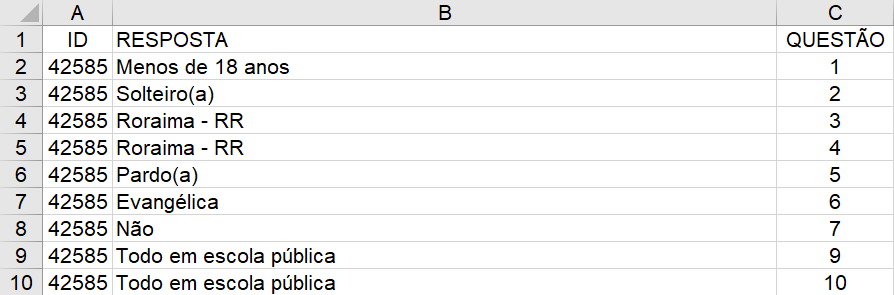
\includegraphics[scale=0.65]{Figuras/Formato_errado.png}
	\end{center}
    \legend{Fonte: Próprio autor.}
\end{figure}

\par
\textcolor{red}{Para poder começar com a utilização desses dados, foi necessário transformar toda a tabela para um formato apropriado a fim de que os aplicativos do software WEKA os suporte. De início foi feito colunas para cada número do questionário através das funções de filtro e concatenação fornecida pelo Excel, e as linhas abaixo delas seriam as respostas de cada candidato para aquela coluna especifica, como demonstrado na Figura 20. A coluna de ID foi removida já que não era necessário para a mineração, entretanto, ela foi necessária na geração de uma coluna nova rotulada de Aprovado que foi obtida através de duas tabelas contendo informações dos candidatos geral e dos candidatos aprovados.}

\par
\begin{figure}[!htp]
	\begin{center}
    \caption{\label{fig:waveform_fig} Tabela depois de formatada.}
	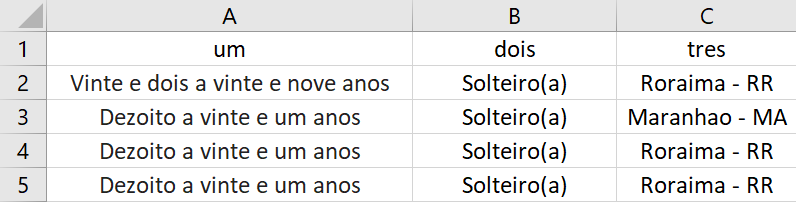
\includegraphics[scale=0.65]{Figuras/Formato_certo.png}
	\end{center}
    \legend{Fonte: Próprio autor.}
\end{figure}

\par
\textcolor{red}{O motivo dessa formatação demonstrado na Figura 20 é que o WEKA identifica a primeira linha como os atributos e as linhas subsequentes os dados relacionados a esses atributos. Como o software trabalha com formato de arquivo próprio denominado \textit{Atribute-Relation File Format} (arff), foi preciso salvar o arquivo que estava no formato xlsx para o formato csv (que separa colunas por ponto e vírgula), pois, o próprio WEKA converte esse tipo de arquivo para o tipo de arquivo que ele trabalha, o arff.}

\par
\textcolor{red}{Também foi necessário se fazer algumas alterações nas informações de dentro da tabela para que depois da conversão não viesse a ocorrer algum erro nos dados. Alterações essas como a remoção de acentos identificados nas informações da tabela, pois, os arquivos no WEKA segundo \citeonline{Amaral2016}, se encontram no formato ASCII que não suportam caracteres acentuados, outra alteração foi a de transformar números para textos, pois, o tipo de dado em cada coluna só pode ser \textit{numeric nominal}, \textit{string} ou \textit{date}, e por fim, a última alteração foi a da remoção de virgulas encontradas nos dados, pois, para converter um arquivo csv no formato arff, o WEKA identifica as virgulas como as colunas que separam os dados.}

\par
\textcolor{red}{A última alteração que precisou ser feita foi da transformação dos ponto e vírgula para somente virgula, pois, o Excel ao transformar um arquivo em xlsx para csv, ele faz com a separação da coluna seja feita por ponto e vírgula o que acaba ocasionando erros e inconsistência nos dados quando o arquivo é convertido do csv para o arff, pois, o WEKA considera o caractere virgula como a representação das colunas que separam os dados. Após ter feito todos esses processos que foram mencionados anteriormente, a conversão do arquivo foi um sucesso, não tendo sido encontrado nenhum problema e inconsistência nos dados que possam ocasionar erro durante o processo de mineração.}


\subsection{Arquivo ARFF}

\par
\textcolor{red}{Após todo o processo de conversão, internamente, o arquivo arff possui duas seções principais: um cabeçalho e uma área de dados. Segundo \citeonline{Amaral2016}, um cabeçalho deve possuir o nome do conjunto de dados através do atributo relação, no caso, o nome do conjunto deve ser acompanhado pela marca @relation seguido com os atributos que compõem a relação com a marca @attribute. Como podemos ver representado na Figura 21 o arquivo utilizado para a mineração de dados, onde a marca @relation traz o nome do conjunto: Vestibulando de 2017. Se tem no total 34 atributos marcados por @relation, sendo todos os atributos do tipo categórico.} 

\par
\begin{figure}[!htp]
	\begin{center}
    \caption{\label{fig:waveform_fig} Cabeçalho do arquivo arff.}
	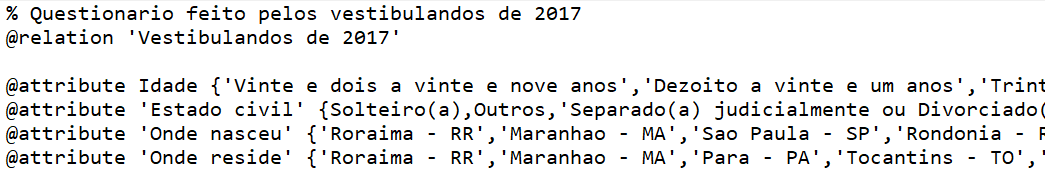
\includegraphics[scale=0.57]{Figuras/arquivo_arff.png}
	\end{center}
    \legend{Fonte: Próprio autor.}
\end{figure}

\par
\textcolor{red}{A seção de área de dados tem o seu início definido pela marca @data, onde os dados dessa área são posicionados em linhas, separados por vírgulas, na mesma ordem em que foram colocados os atributos que teve como um total de 8.571 linhas (que é a quantidade de inscritos que responderam o questionário ), como representado na Figura 22.}

\par
\begin{figure}[!htp]
	\begin{center}
    \caption{\label{fig:waveform_fig} Área de Dados do arquivo arff.}
	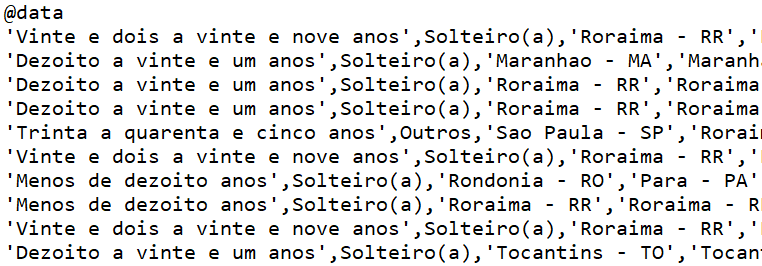
\includegraphics[scale=0.60]{Figuras/arquivo_arff_2.png}
	\end{center}
    \legend{Fonte: Próprio autor.}
\end{figure}


\subsection{Selecionando os atributos}

\par
\textcolor{red}{Para muitos classificadores, quando recebem uma grande quantidade de atributos, acaba ocasionando um efeito de superajustes nos modelos que os tona ineficiente, segundo \citeonline{Amaral2016}, esse efeito é conhecido como maldição da dimensionalidade. Esse mesmo tipo de problema ocorre com os atributos dos dados socioeconômicos fornecidos para esse trabalho, no caso, para o algoritmo de classificação J48 que é utilizado. Para contornar esse problema foi utilizado a técnica de seleção de atributos que o Explorer do software WEKA disponibiliza, no qual descobre quais atributos são mais relevantes para a melhor generalização do modelo.}

\par
\textcolor{red}{Para a execução da seleção de atributo no WEKA, é preciso selecionar o avaliador de atributo (\textit{Attribute Evaluator}) e o método de busca (\textit{Search Method}). Como demonstrado na Figura 23, o método de avaliação escolhido foi a opção \textit{CfsSubetEval}, onde ele considera a capacidade preditiva individual de cada recurso, diretamente com o grau de redundância entre eles e para o método de busca foi escolhido a opção \textit{GreedyStepwise} que faz uma busca avançada tanto pra frente quanto pra trás através do espaço de subconjuntos de atributos e também pode criar uma lista classificada de atributos, fazendo que sejam registrados na o ordem em que elas foram selecionadas \cite{WEKA}. Além do que, segundo \citeonline{Amaral2016}, esse método de busca é compatível com o algoritmo de avaliação de atributo escolhido. }

\par
\begin{figure}[!htp]
	\begin{center}
    \caption{\label{fig:waveform_fig} Representação do avaliador de atributo e método de busca.}
	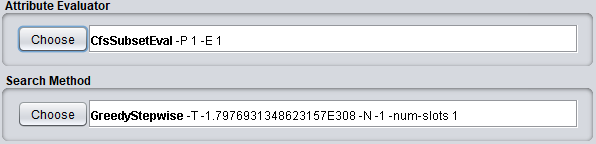
\includegraphics[scale=0.90]{Figuras/Avaliador_de_atributo.png}
	\end{center}
    \legend{Fonte: Próprio autor.}
\end{figure}

\par
\textcolor{red}{Nos primeiros testes de seleção, foi optado de usar tanto a opção de treino para todo o conjunto quanto a opção de \textit{cross-validation} com um número 10 de fold, nos 33 atributos relacionado ao atributo Aprovado, para os dois casos, o atributo mais relevante para a classificação era o estado onde o vestibulando residia como demonstrado na Figura 24. Então, para resolver esse problema, teve que ser feita a remoção de alguns atributos que eram desnecessários para esta pesquisa como o melhor horário para cursar a universidade, o que esperar do curso, como soube do processo seletivo e entre outros, depois de ter feito a remoção, de 33 atributos sobraram somente 22 para serem aplicados no algoritmo de seleção do WEKA.}

\par
\begin{figure}[!htp]
	\begin{center}
    \caption{\label{fig:waveform_fig} Resultado da seleção de atributos utilizando o método cross-validation para o treino.}
	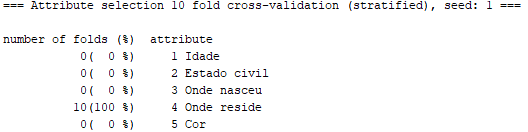
\includegraphics[scale=0.99]{Figuras/33_atributos.png}
	\end{center}
    \legend{Fonte: Próprio autor.}
\end{figure}



\par
\textcolor{red}{Mas antes de ser aplicado a técnica de seleção, foi feito os seguintes testes, primeiro foi utilizado os atributos para o teste de seleção que os autores dos trabalhos correlatos que teve como base para este projeto. Foi utilizado os 4 atributos mais importantes para a pesquisa que os autores \citeonline{LeandroSilva2014} selecionaram, mais os 9 atributos de 25 que \citeonline{Simon2017} selecionaram, entretanto, apena 2 de 9 atributos foi utilizado para o teste, por que, os outros 7 eram dados de escolas que o INEP fornecia, diferente dos dados que a CPV forneceu. Juntando os atributos que os dois trabalhos selecionaram, teve no total de 4 atributos como base: a escola que cursou o ensino médio, escolaridade da mãe, renda mensal familiar e quantidade de pessoas que moram com a pessoa.}

\par\textcolor{red}{Aplicando o algoritmo de seleção nesses 4 atributos, teve como resultado, que apenas 3 deles estavam acima do 70\%  (mais relevantes para a classificação) como demonstrado na Figura 25.}

\par
\begin{figure}[!htp]
	\begin{center}
    \caption{\label{fig:waveform_fig} Resultado da seleção de atributos do 4 atributos utilizados.}
	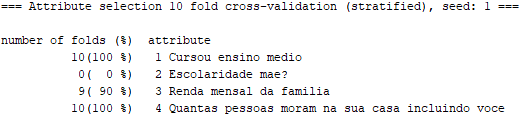
\includegraphics[scale=0.99]{Figuras/4_atributos.png}
	\end{center}
    \legend{Fonte: Próprio autor.}
\end{figure}

\par
\textcolor{red}{Depois do teste que foi feito com os atributos base, foi acrescentado mais um atributo ao teste, para poder mais uma vez executar a seleção de atributos e depois analisar os resultados, isso foi feito sucessivamente até chegar aos 22 atributos. Depois de todo o processo de teste, no final, teve como resultado que os atributos mais relavantes (que ultrapassavam de 70\%) que foram obtidos nos dados fornecidos eram praticamente diferentes dos dados selecionados para o teste base, como demonstrado na Figura 26.}

\par
\begin{figure}[!htp]
	\begin{center}
    \caption{\label{fig:waveform_fig} Resultado final dos testes de seleção.}
	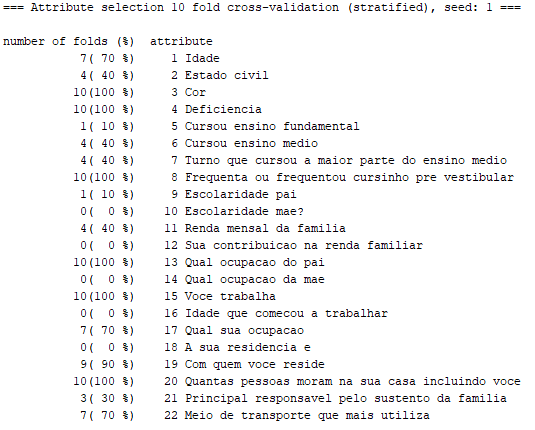
\includegraphics[scale=0.90]{Figuras/22_atributos.png}
	\end{center}
    \legend{Fonte: Próprio autor.}
\end{figure}

\par
\textcolor{red}{Então, os dados que foram obtidos como mais relevantes pela seleção de atributos do Explore do WEKA, que serão utilizados para a classificação, foram: idade do candidato, a cor de pele, se possui alguma deficiência, se frequentou algum cursinho pré-vestibular, ocupação do pai, se o candidato trabalhava, a ocupação do candidato, com quem ele residia, quantidades de pessoas que moram com ele e por último o meio de transporte que ele utiliza.}

\subsection{Problemas de classe rara}

\par
\textcolor{red}{É normal em alguns casos de quando se vai minerar algum dado ocorra o problema de classe rara, que segundo \citeonline{Amaral2016}, explica que quando uma instancia de uma classe é predominante do que outra instancia de outra classe, a consequência é de que o modelo aprenderá somente as características da classe dominante, enquanto ele falhará em classificar novas instancias da outra classe, pelo motivo de ela ser uma classe rara. É o que acontece nos dados desse trabalho, especificamente no atributo de Aprovado que tem no total de 8571 instancias, possuindo a classe Sim com 7784 instancias (81\%) e a Classe Nao com 787 instancias (9\%) como demonstrado na Figura 24.}

\par
\begin{figure}[!htp]
	\begin{center}
    \caption{\label{fig:waveform_fig} Representação do atributo Aprovado com as suas duas classes Sim e Nao.}
	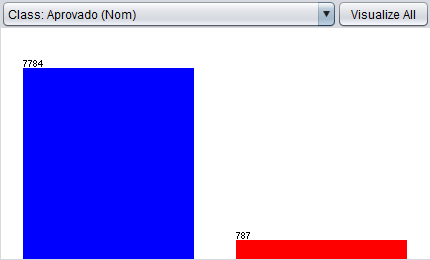
\includegraphics[scale=0.90]{Figuras/Atributo_aprovado.png}
	\end{center}
    \legend{Fonte: Próprio autor.}
\end{figure}

\par
\textcolor{red}{Segundo \citeonline{Amaral2016}, a solução mais comum para esse tipo de problema é de utilizar as técnicas de estratificação. No software WEKA, para métodos supervisionado, possui 4 técnicas de estratificação para instancias, no caso, a que foi utilizada para resolver esse tipo de problema foi a técnica SpreadSubsample, pois, segundo o site do software \citeonline{WEKA} esse tipo de filtro gera uma subamostra aleatória de um conjunto de dados, permitindo especificar o \textit{spread} máximo entre a classe mais rara e a classe mais comum, ou seja, balanceado o conjunto de dados dessas duas classe.}

\par
\textcolor{red}{No filtro SpreadSubsample a opção escolhida para a distributionSpread (\textit{spread} máximo distribuição de classe) foi de 1 que representa a opção de distribuição uniforme que é demonstrada na Figura 25. Depois de ser aplicado esse filtro na classe de Aprovado, tem como resultado um conjunto de dados balanceado tanto para a classe mais comum (Sim) como a classe mais rara (Nao), como representada na Figura 26.}

\par
\begin{figure}[!htp]
	\begin{center}
    \caption{\label{fig:waveform_fig} Representação da configuração  do filtro SpreadSubsample.}
	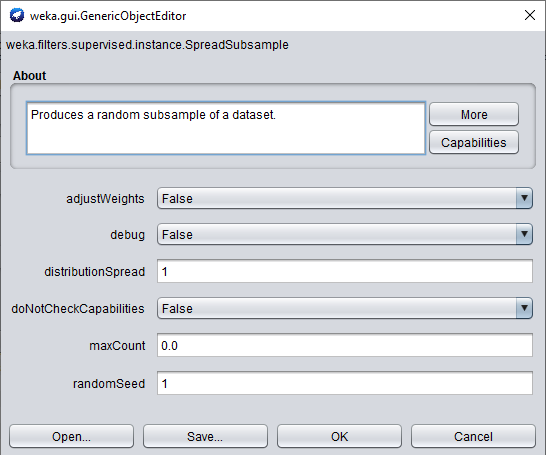
\includegraphics[scale=0.99]{Figuras/SpreadSubsample.png}
	\end{center}
    \legend{Fonte: Próprio autor.}
\end{figure}

\par
\begin{figure}[!htp]
	\begin{center}
    \caption{\label{fig:waveform_fig} Resultado do balanceamento do atributo Aprovado.}
	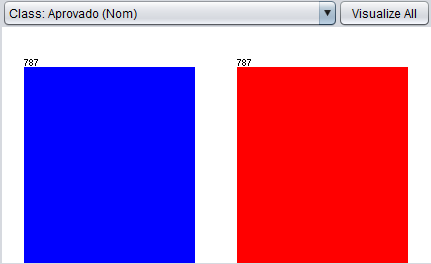
\includegraphics[scale=0.90]{Figuras/Atributo_aprovado_balanceado.png}
	\end{center}
    \legend{Fonte: Próprio autor.}
\end{figure}

